\documentclass[10pt]{article}
\usepackage[utf8]{inputenc}
\usepackage{geometry}
\usepackage[sort]{natbib}
\usepackage{pxfonts}
\usepackage{graphicx}
% \graphicspath{ {./figures-low/} }
\graphicspath{ {./figures-default/} }
\usepackage{setspace}
\usepackage{hyperref}
\usepackage{lineno}
\usepackage{authblk}
\usepackage{pdflscape}
\usepackage{rotating}
\usepackage{multirow}
\usepackage[online,flushleft]{threeparttable}
\usepackage{booktabs}

\doublespacing
\linenumbers

\title{\textit{Supplementary materials for:} The psychological arrow of time drives temporal asymmetries in inferring unobserved past and future events}
\author[1]{Xinming Xu}
\author[2]{Ziyan Zhu}
\author[1, $\star$]{Jeremy R. Manning}
\affil[1]{Dartmouth College, Hanover, NH, USA}
\affil[2]{Peking University, Beijing, China}
\affil[$\star$]{Address correspondence to jeremy.r.manning@dartmouth.edu}

\begin{document}
\maketitle

\renewcommand{\thefigure}{S\arabic{figure}}
\renewcommand{\thetable}{S\arabic{table}}


\begin{table}[]
\caption{\textbf{Stimuli description.}}
\begin{center}
\resizebox{\textwidth}{!}{
\begin{threeparttable}
\begin{tabular}{rrrrlll}
\toprule
\multirow{2}{*}{Storyline} &
  \multirow{2}{*}{Segment} &
  \multirow{2}{*}{Episode} &
  \multirow{2}{*}{Duration (s)} &
  \multirow{2}{*}{Main characters} &
  \multicolumn{2}{l}{Number of events\tnote{a}} \\ \cmidrule(l){6-7} 
  &    &   &     &                                & Onscreen      & Offscreen\tnote{b} \\ \midrule
1 & 1  & 1 & 105 & Beth, Sheila, Rob, Leo         & 4             & 7         \\
1 & 2  & 1 & 172 & Beth, Sheila, Rob, Leo         & 7 {[}1{]}     & 3         \\
1 & 3  & 1 & 70  & Beth, Sheila, One neighbor     & 6             & 2         \\
1 & 4  & 1 & 135 & Beth, Sheila                   & 8 {[}1{]}     & 1         \\
1 & 5  & 1 & 90  & Beth, Rob, April               & 8             & 4         \\
1 & 6  & 1 & 188 & Beth, Rob                      & 6 {[}2{]}     & 1         \\
1 & 7  & 1 & 91  & Beth, Sheila                   & 5 {[}1{]}     & 2         \\
1 & 8  & 1 & 142 & Beth, April                    & 4 (1) {[}2{]} & 3 (1)     \\
1 & 9  & 2 & 134 & Beth, April                    & 4 {[}2{]}     & 1         \\
1 & 10 & 2 & 58  & Beth                           & 3 {[}1{]}     & 6 {[}1{]} \\
1 & 11 & 2 & 159 & Beth, Rob                      & 9             &           \\
2 & 1  & 1 & 70  & Simone, Karl                   & 3 {[}1{]}     & 6         \\
2 & 2  & 1 & 119 & Simone, Karl, Naomi, Tommy     & 4 {[}1{]}     & 2         \\
2 & 3  & 1 & 58  & Simone, Karl, Tommy            & 4             & 2         \\
2 & 4  & 1 & 102 & Simone, Karl                   & 4             & 6         \\
2 & 5  & 1 & 134 & Simone, Karl, Tommy            & 6 (3) {[}1{]} & 3         \\
2 & 6  & 1 & 81  & Simone, Karl, Neighbors, Wanda & 4 (1)         & 6         \\
2 & 7  & 1 & 194 & Simone, Tommy                  & 8             & 3         \\
2 & 8  & 2 & 101 & Simone, Karl                   & 3 (1)         & 1         \\
2 & 9  & 2 & 86  & Simone, Tommy                  & 4 {[}1{]}     & 3         \\
2 & 10 & 2 & 232 & Simone, Karl                   & 6 {[}1{]}     & 3         \\
2 & 11 & 2 & 189 & Simone, Naomi, Tommy           & 7 (1) {[}1{]} &           \\ \bottomrule
\end{tabular}
\begin{tablenotes}
\item[a] Number of partial events (see methods) shown in parentheses; number of summary events shown in square brackets.
\item[b] Offscreen events happened between the current segment and the next segment.
\end{tablenotes}
\end{threeparttable}
}
\end{center}
\end{table}

\begin{figure}[tp]
    \centering
    \includegraphics[width=\textwidth]{supp1.pdf}
    \caption{\textbf{Mean proportion of target events hit (A), precision (B), and convergence (C) as a function of number of segments watched in each storyline, in participants' uncued and character-cued retrodictions and predictions.} Grey lines represent the least squares fits.}
    \label{fig:supp1}
\end{figure}

\begin{figure}[tp]
    \centering
    \includegraphics[width=\textwidth]{supp2.pdf}
    \caption{\textbf{Mean number of events hit for each event type, in participants' uncued and character-cued retrodictions and predictions, averaged across just-watched segments.}}
    \label{fig:supp2}
\end{figure}

\begin{figure}[tp]
    \centering
    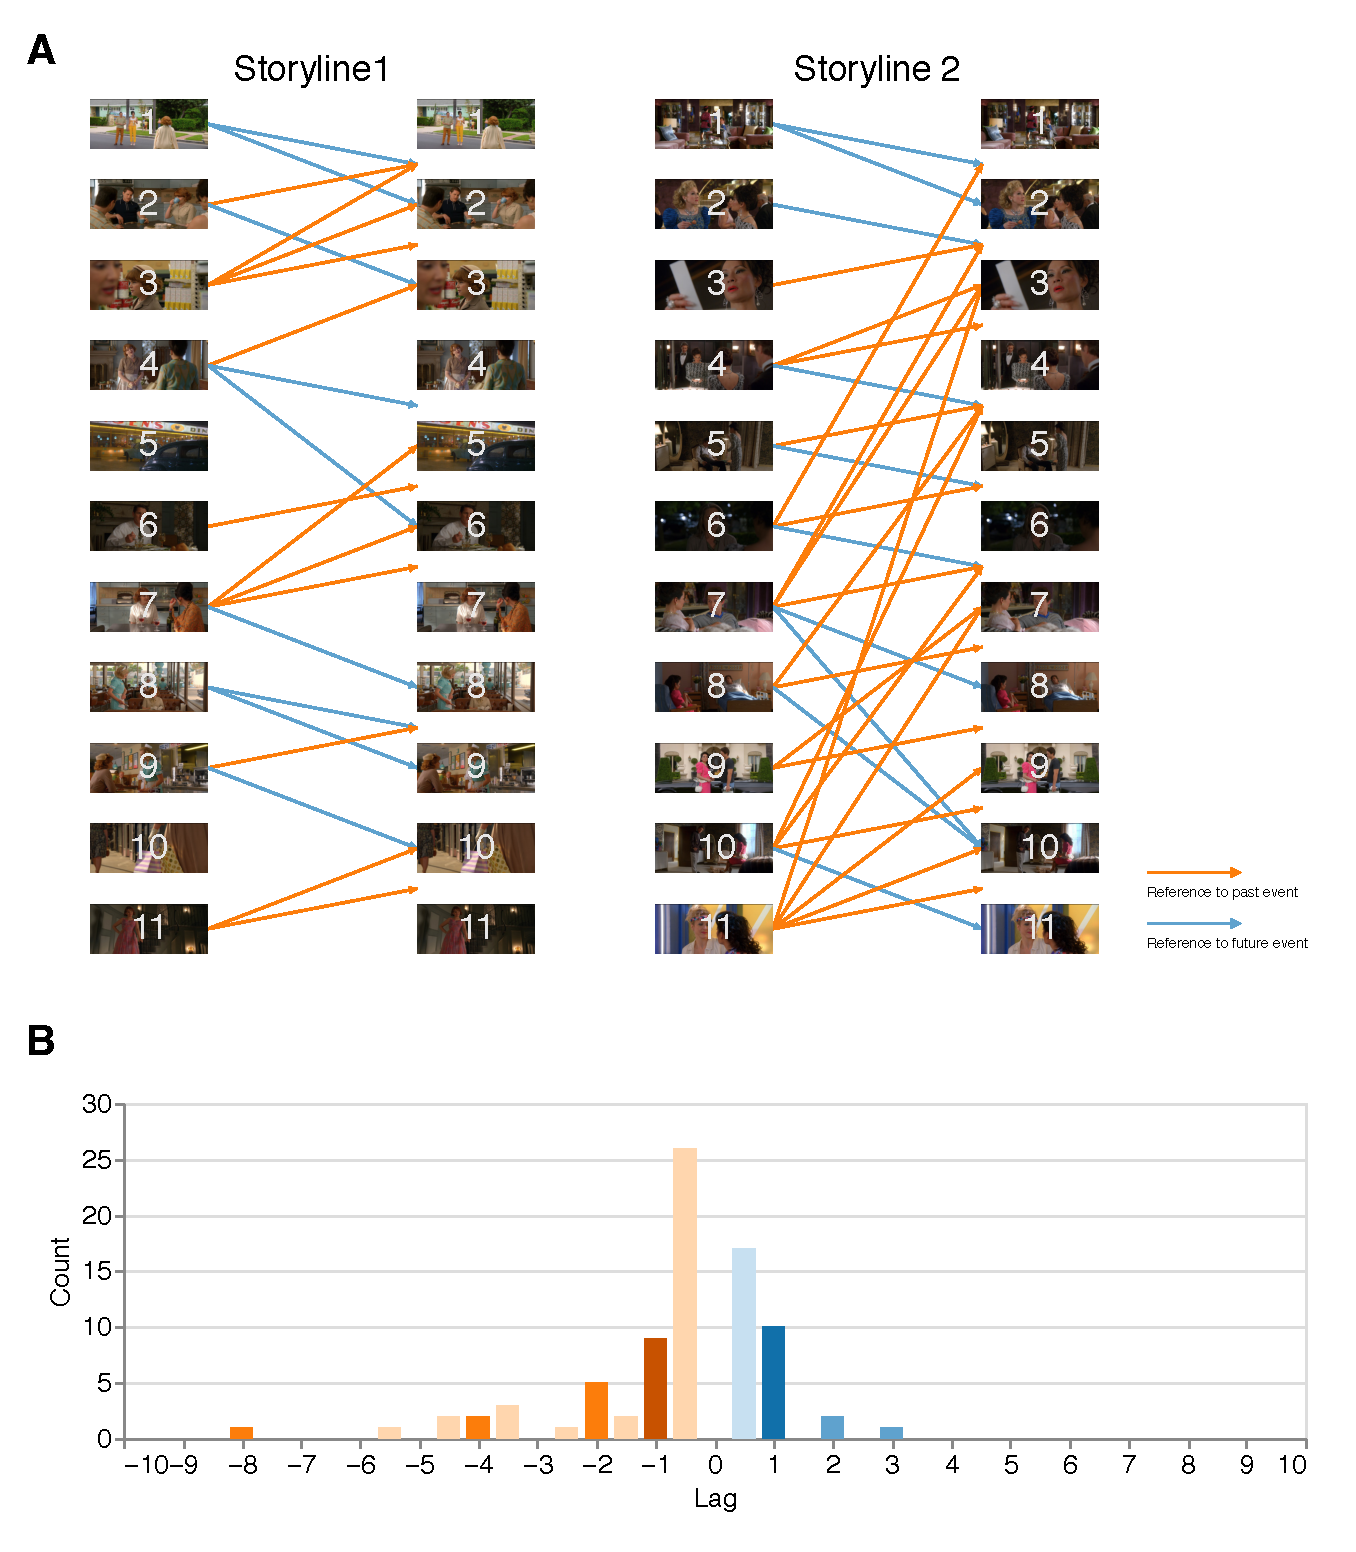
\includegraphics[width=\textwidth]{supp3.pdf}
    \caption{\textbf{(A)} References in each storyline. \textbf{(B)} Distribution of reference lags.}
    \label{fig:supp3}
\end{figure}


\end{document}